\section{Протокол оценки}
\label{sec:proto}

Что считать выигрышем, решается до эксперимента. Иначе за два месяца можно уехать сколь угодно далеко.

\subsection{Три уровня строгости разбиения}

\emph{Случайное пятикратное} --- верхняя граница, полезна только для отладки. Оптимистичнее кластерного
примерно вдвое по $R^2$.

\emph{Кластерное по Бутине при пороге 0.35} --- рабочий режим, все числа этого документа получены на нём.
Соединения группируются по сходству, и целый кластер целиком уходит в отложенный фолд, так что модель
не может узнать соединение по его близкому родственнику в обучении.

\emph{Разбиение под дизайн теста} --- ближе всего к реальности. Псевдотестовый фолд строится тем же
алгоритмом, что и настоящий тест: берём хит из обучающей выборки, забираем его 10 ближайших соседей,
держим всю серию снаружи.

\subsection{Насколько наша проверка похожа на тест}

Прежде чем отбирать модели, надо спросить: наша кросс-валидация вообще такой же трудности, как тест?
Мера простая --- сходство соединения с ближайшим к нему обучающим.

\begin{figure}[htbp]\centering
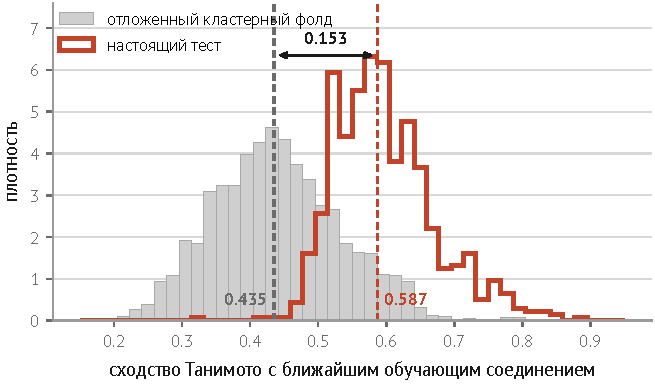
\includegraphics{fig/nnsim}
\caption{Насколько далеко проверяемое соединение от того, что модель видела. Разрыв медиан 0.153,
и он идёт в неожиданную сторону: наша проверка труднее теста.}
\label{fig:nnsim}
\end{figure}

У отложенного кластерного фолда медиана 0.435 и доля соединений со сходством выше 0.7 равна половине
процента. У настоящего теста медиана 0.587, и таких соединений каждое десятое.

Приятная половина: 0.767 --- оценка снизу, на лидерборде должно быть лучше. Неприятная: мы отбираем
модели по способности экстраполировать на чужую химию, а тест награждает за интерполяцию внутри серии
аналогов. Это разные умения, и лучшая по нашей сетке модель не обязана быть лучшей там. Эту дыру
закрывает разбиение под дизайн теста, и теперь у него есть цена, выраженная числом.

\subsection{Устойчивость к разбиению}

Все числа регрессионного трека изначально стояли на одном разбиении --- кластеры Бутины, раскиданные
по фолдам генератором с зерном ноль. Парный бутстрап покрывал случайность выборки соединений, но не
случайность самого разбиения. Прогон на других зёрнах меняет только то, как кластеры распределяются
по пяти фолдам; кластеризация, признаки, гиперпараметры и код те же.

\begin{figure}[htbp]\centering
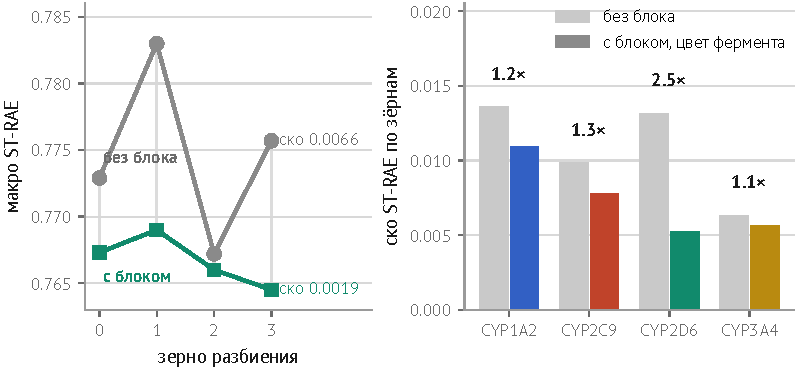
\includegraphics{fig/seeds}
\caption{Слева --- макро-ST-RAE на четырёх зёрнах разбиения. Справа --- стандартное отклонение по этим
четырём зёрнам, по ферментам. Механистический блок снижает зависимость от разбиения в 3.4 раза
по макро, и падение сосредоточено на 2D6.}
\label{fig:seeds}
\end{figure}

Абсолютный уровень плавает: 0.7729, 0.7830, 0.7672, 0.7757 для набора без механистического блока.
Стандартное отклонение 0.0066, размах 0.0158 --- больше, чем весь эффект, ради измерения которого
строилась абляционная сетка. Любое число вида «макро 0.767» без указания разбиения имеет точность
до первого знака после запятой, не до третьего.

Направление держится: разность отрицательна на всех четырёх зёрнах ($-0.0056$, $-0.0140$, $-0.0012$,
$-0.0112$), Спирмен растёт тоже на всех четырёх, а на 2D6 от $+0.033$ до $+0.052$. Бутстрап на одном
разбиении накрывал ноль; четыре разбиения показывают, что знак устойчив, хотя величина гуляет в десять раз.

Самое интересное здесь в разбросах, а не в средних. Набор без блока имеет по зёрнам разброс 0.0066,
с блоком --- 0.0019, в 3.4 раза меньше. По ферментам эффект сосредоточен там, где и должен: на 2D6
разброс падает с 0.0132 до 0.0052, а на 3A4 почти не меняется.

Похоже, двадцать восемь механистических чисел дают модели опору, не зависящую от того, какие аналоги
попали в обучающие фолды. Фингерпринт такой опоры не даёт: он узнаёт соединение по соседям, и когда
соседи уезжают в отложенный фолд, узнавание рассыпается. Главная польза блока, видимо, в этом,
а не в приросте среднего.

Протокол из-за этого меняется. Любое сравнение вариантов идёт на фиксированном наборе из нескольких
разбиений и отчитывается разностью на каждом плюс разбросом. Одно разбиение годится для отладки
и не годится для решения, что отправлять.

\subsection{Парный бутстрап}

Любое сравнение двух вариантов --- только на одном и том же разбиении и с парным бутстрапом
по соединениям: 2000--3000 пересборок, для каждой обе метрики пересчитываются на одной и той же
пересобранной выборке, докладывается распределение разности и доля пересборок, где стало хуже.
Разность без интервала не является результатом.

Для макро надо ресэмплить соединения общей таблицы, а потом для каждого фермента брать те из них,
у кого есть метка --- так сохраняется корреляция между ферментами. Считать четыре независимых бутстрапа
и усреднять нельзя.

\subsection{Сетка абляций}

Каждая строка снимается с парным бутстрапом относительно предыдущей, на нескольких зёрнах.

\begin{enumerate}
\item Фингерпринт и дескрипторы, бустинг. Базовая линия.
\item Предобученный энкодер вместо ручных признаков, одна голова на эндпойнт.
\item Плюс коррегионализация \eqref{eq:icm}.
\item Плюс механистический блок и канал артефактов пробы.
\item Плюс скрининг через \eqref{eq:scr}: главная проверка всей идеи.
\item Плюс Emax и плечо с преинкубацией в общее правдоподобие.
\item Плюс ансамбль и конформная калибровка.
\item Плюс решающий слой: отдельно для регрессии, отдельно для MCC.
\item Плюс трансдуктивный слой.
\end{enumerate}

Строка 5 --- точка, на которой конструкция оправдывается или не оправдывается. Обязательный контроль
к ней: сильная многозадачная базовая линия на тех же признаках и том же энкодере, обученная на одних
метках кривых. Если совместное правдоподобие её не обыгрывает, это отрицательный результат, и он идёт
в отчёт как есть.
